\documentclass[oneside, zh]{nfuthesis}
\usepackage{enumitem}
\usepackage{times}
\usepackage{verbatim}
\usepackage{color}
\usepackage{url}
\usepackage{graphicx}
\usepackage{array}
\usepackage{pdfpages}  % include inserted .pdf to page no.
\usepackage{wallpaper} % watermark
\usepackage{amsmath}   % math 
% \usepackage{mathtools} % math, 'mathtools' is an extention of 'amsmath'

% Format the refs
\usepackage[sort, square, comma, compress]{natbib} % 參考文獻引用。排序、方括號、逗號分隔、壓縮。
\usepackage[hidelinks]{hyperref}

% For Cross ref
\usepackage{xr}

% For the tree
\usepackage{tikz}
\usepackage{tikz-qtree}

% For code display
\usepackage{listings}

% For the APA table
\usepackage{adjustbox}
\usepackage{multirow,booktabs,setspace,caption}
\usepackage{rotating}
\usepackage{dcolumn}
\newcolumntype{z}{D{.}{.}{3}} % for decimal dot alignment

% Remove caption separator of tables and figures
\captionsetup[table]{labelsep=space}
\captionsetup[figure]{labelsep=space}

% For hyperlink
\usepackage{hyperref}

% For barchart
\usepackage{pgfplots}
\pgfplotsset{compat=1.12}

% For setting counters of figure and table
\usepackage{chngcntr}

% Using the tex-text mapping for ligatures etc.
\defaultfontfeatures{Mapping=tex-text}

% Set the default fonts
\setmainfont{Times New Roman}
\setCJKmainfont{TW-Kai} % modify for overleaf service

% Your information goes here
\input{nctuvars}

\begin{document}

\hypersetup{pageanchor=false}

\frontmatter
\pagenumbering{gobble}

% 此處不自動產生交大封面改採插入pdf封面故註解
% \makecover

% 以插入pdf檔方式加入封面及書名頁
\includepdf[pages={1}]{pdfs/cover.pdf}
\includepdf[pages={1}]{pdfs/first_page.pdf}

% 開始編羅馬數字頁碼
\clearpages
\setcounter{page}{1}
\hypersetup{pageanchor=true}
\pagenumbering{roman}
\phantomsection

% 插入論文審定書 著作權審定書等等
\addcontentsline{toc}{chapter}{中文論文口試委員會審定書}

\includepdf[pages={1}, pagecommand={}]{pdfs/ch.pdf}
\addcontentsline{toc}{chapter}{Thesis Certificate}
\includepdf[pages={1}, pagecommand={}]{pdfs/en.pdf}
\addcontentsline{toc}{chapter}{論文著作權授權書}
\includepdf[pages={1}, pagecommand={}]{pdfs/copyright.pdf}

% 論文浮水印 如不需要浮水印時註解此行
% 論文浮水印
\CenterWallPaper{0.8}{images/watermark_nfu.jpg}
\setlength{\wpXoffset}{0 cm}
\setlength{\wpYoffset}{0 cm}


% 摘要、致謝
\input{abstract}
\begin{acknowledgementszh}

感謝萊斯利·蘭波特(Leslie Lamport)博士發明的 \LaTeX\ ,讓我不用苦惱於Word的排版。

\end{acknowledgementszh}

% 自行決定是否需英文誌謝
% \begin{acknowledgementsen}
% This is English line spacing test. You should see double spacing text.
% This is English line spacing test. You should see double spacing text.
% This is English line spacing test. You should see double spacing text.
% This is English line spacing test. You should see double spacing text.
% This is English line spacing test. You should see double spacing text.
% This is English line spacing test. You should see double spacing text.
% This is English line spacing test. You should see double spacing text.
% This is English line spacing test. You should see double spacing text.

% I'm glad to thank\ldots 
% \end{acknowledgementsen}



% Table of Content
\clearpages
\tableofcontents

% List of Figures
\clearpages
\listoffigures

% List of Tables
\clearpages
\listoftables

\mainmatter

% tables and figures counter within chapter
\counterwithin{table}{chapter}
\counterwithin{figure}{chapter}

% Math equations counter winout chapter
\counterwithout{equation}{chapter}

% Your thesis goes here
\chapter{緒論}
\label{c:intro}

\section{研究動機}

文獻\cite{test2021}指出... ...。測試文字測試文字測試文字測試文字測試文字測試文字測試測試文字測試文字測試文字測試文字測試文字測試文字測試

測試文字測試文字測試文字測試文字測試文字測試文字測試文字測試文字測試文字測試文字測試文字測試文字測試文字測試文字測試文字測試文字測試文字測試文字測試文字測試文字測試文字測試文字測試文字測試文字測試文字測試文字測試文字測試文字測試文字測試文字

\section{研究背景}
\subsection{測試測試}

\section{研究目標}

\begin{enumerate}
\item 測試 
\item 測試 
\item 測試
\item 想辦法畢業
\end{enumerate}

\section{研究問題}
整合上述,本研究要想辦法畢業。

\section{研究重要性} 

畢業

\chapter{文獻探討}

\section{測試}

測試文字測試文字測試文字\cite{test2018,test2019}。

\chapter{研究方法}
\section{研究設計與流程}

測試文字測試文字測試文字測試文字測試文字測試文字測試文字測試文字測試文字測試文字測試文字測試文字測試文字測試文字測試文字測試文字測試文字測試文字測試文字測試文字測試文字測試文字測試文字測試文字測試文字測試文字測試文字測試文字測試文字測試文字測試文字測試文字測試文字測試文字測試文字測試文字測試文字測試文字測試文字測試文字測試文字測試文字測試文字測試文字測試文字測試文字測試文字測試文字測試文字測試文字測試文字測試文字測試文字測試文字測試文字測試文字測試文字測試文字測試文字測試文字測試文字測試文字測試文字測試文字測試文字測試文字測試文字測試文字測試文字測試文字測試文字測試文字測試文字測試文字測試文字測試文字測試文字測試文字測試文字測試文字測試文字測試文字測試文字測試文字測試文字測試文字測試文字測試文字測試文字測試文字測試文字測試文字測試文字測試文字測試文字測試文字測試文字測試文字測試文字測試文字測試文字測試文字測試文字測試文字測試文字測試文字

測試文字測試文字測試文字測試文字測試文字測試文字測試文字測試文字測試文字測試文字測試文字測試文字測試文字測試文字測試文字測試文字測試文字測試文字測試文字測試文字測試文字測試文字測試文字測試文字測試文字測試文字測試文字測試文字測試文字測試文字測試文字測試文字測試文字測試文字測試文字測試文字測試文字測試文字測試文字測試文字測試文字測試文字測試文字測試文字測試文字測試文字測試文字測試文字測試文字測試文字測試文字測試文字測試文字

圖\ref{i:debug}顯示了遇到機械機構問題時採用的解法流程圖。
\begin{figure}[!htbp]
\centering

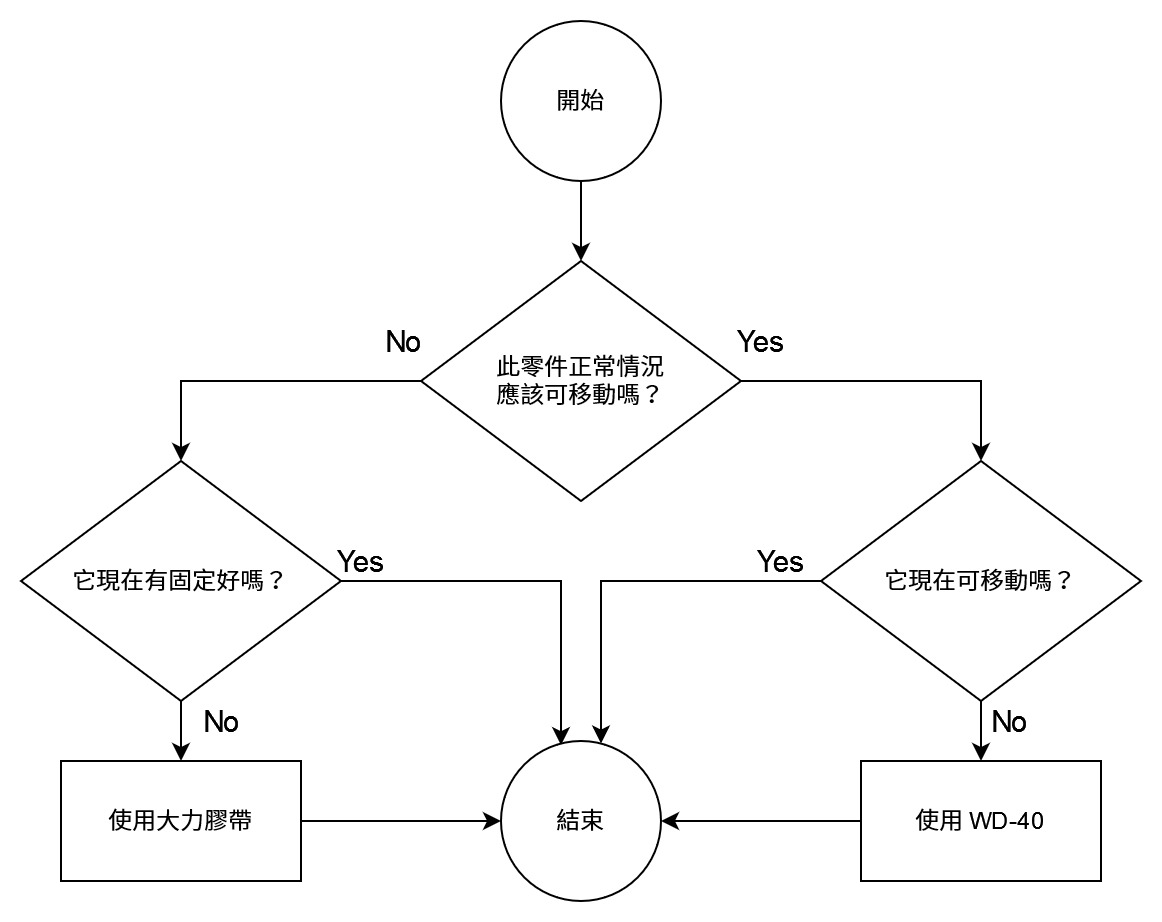
\includegraphics[width=.85\columnwidth]{images/debug.jpg}
\caption{機械問題除錯流程圖}
\label{i:debug}

\end{figure}


樹範例如~\ref{i:tree}
\begin{figure}[!htbp]
\centering

\tikzset{every tree node/.style={align=center},
    level distance=40pt,
    sibling distance=6pt}
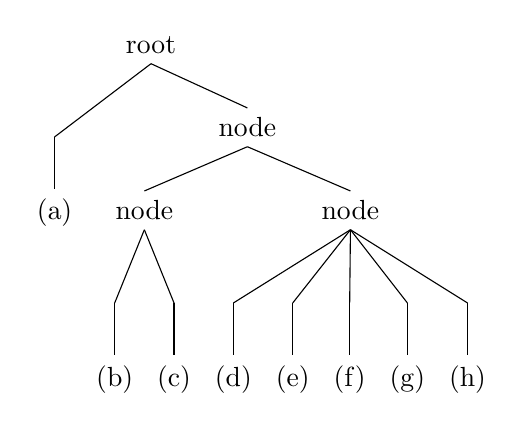
\begin{tikzpicture}
\Tree[.root
       [ (a) ]
       [.node
         [.node
           [ (b) ]
           [ (c) ]
         ]
         [.node
           [ (d) ]
           [ (e) ]
           [ (f) ]
           [ (g) ]
           [ (h) ]
         ]
       ]
     ]

\end{tikzpicture}

\caption{A tree. }
\label{i:tree}
\end{figure}


長條圖範例如~\ref{i:barchart}
\input{figures/barchart}

本研究分組如表~\ref{t:group}
\input{tables/group}

\chapter{實驗結果}
\label{c:experiment}

\section{描述性統計}

本研究各變數實驗結果之描述性統計(個數、最小值、最大值、平均與標準差)如表~\ref{t:a}。

\begin{table}[htbp]
\centering

\caption{受測者描述性統計}
\label{t:a}

\begin{adjustbox}{max width=0.95\textwidth}
\begin{tabular}{lcccrc} % 對齊

\toprule
變數  & 個數 & 最小值 & 最大值 & 平均數      & 標準差 \\ 
\midrule
背景  & 5   &       &       &  35,856    &       \\
資料A & 84  &       &       &  55        &       \\
資料B & 4   &       &       &  2,033.5   &       \\
\bottomrule
\multicolumn{6}{l}{註:本表的內容是亂打的}

\end{tabular}
\end{adjustbox}
\end{table}


\section{實驗結果分析}

如表~\ref{t:b},以雙獨立樣本t檢定檢驗...

\begin{table}[htbp]
\centering
\caption{測試(N=50)}
\label{t:b}
\begin{adjustbox}{max width=\textwidth}
\begin{tabular}{@{}ccccclrc@{}}
\toprule
 \multirow{2}[3]{*}{樣本} & \multicolumn{2}{c}{測試一} & \multicolumn{2}{c}{測試二} &  &  &  \\ \cmidrule(lr){2-5}
 & 平均 & 標準差 & 平均 & 標準差 & 自由度 & t值 & \textit{p-value} \\ \midrule
Q1 & 3.58 & 1.64 & 3.23 & 1.84 & 48 & -.71 & .47 \\
Q2 & 3.71 & 1.48 & 4.04 & 1.42 & 48 & .80 & .42 \\
Q3 & 5.46 & 2.22 & 6.15 & 1.51 & 40.126 & 1.28 & .20 \\ \bottomrule
\end{tabular}
\end{adjustbox}
\end{table}

如表~\ref{t:c}所示...

\begin{sidewaystable}

\centering
\caption{測試anova(N=50)}
\label{t:c}
\begin{adjustbox}{max width=\textwidth}
\begin{tabular}{@{}crrrrr@{}}

\toprule
\multicolumn{1}{l}{} & \multicolumn{1}{c}{\begin{tabular}[c]{@{}c@{}}G1\\ 測試\\ N=12\\ (M/SD)\end{tabular}} & \multicolumn{1}{c}{\begin{tabular}[c]{@{}c@{}}G2\\ 測試\\ N=12\\ (M/SD)\end{tabular}} & \multicolumn{1}{c}{\begin{tabular}[c]{@{}c@{}}G3\\ 測試\\ N=14\\ (M/SD)\end{tabular}} & \multicolumn{1}{c}{\begin{tabular}[c]{@{}c@{}}G4\\ 測試\\ N=12\\ (M/SD)\end{tabular}} & \multicolumn{1}{c}{\begin{tabular}[c]{@{}c@{}}F\\ (df)\end{tabular}} \\
\midrule
\multicolumn{1}{l}{變數名稱} & \multicolumn{1}{c}{} & \multicolumn{1}{c}{} & \multicolumn{1}{c}{} & \multicolumn{1}{c}{} & \multicolumn{1}{c}{} \\
測試 & (7.25/1.76) & (6.00/1.80) & (6.43/1.91) & (6.42/1.73) & \begin{tabular}[c]{@{}r@{}}1.00\\ (3,46)\end{tabular} \\
測試 & (40.16/12.01) & (40.08/11.13) & (34.35/10.93) & (36.33/7.66) & \begin{tabular}[c]{@{}r@{}}.95\\ (3,46)\end{tabular} \\
測試 & (68.83/14.04) & (68.83/23.37) & (79.21/22.73) & (81.75/30.13) & \begin{tabular}[c]{@{}r@{}}1.05\\ (3,46)\end{tabular} \\
測試 & (39.25/74.65) & (10.66/91.36) & (30.71/38.42) & (18.00/90.86) & \begin{tabular}[c]{@{}r@{}}.19\\ (3,46)\end{tabular} \\
測試 & (1.37/.42) & 高(1.58/.82) & (1.11/.62) & 低(.80/.63) & \begin{tabular}[c]{@{}r@{}}3.33*\\ (3,46)\end{tabular} \\
測試 & (04.66/12.66) & (39.83/11.26) & (71.92/29.64) & (39.50/19.43) & \begin{tabular}[c]{@{}r@{}}.71\\ (3,46)\end{tabular} \\
測試 & (4.84/1.21) & (5.14/1.41) & (4.59/1.12) & (4.78/1.45) & \begin{tabular}[c]{@{}r@{}}.40\\ (3,46)\end{tabular} \\
測試 & (10.45/34.43) & (05.12/41.36) & (87.46/34.60) & (95.20/30.74) & \begin{tabular}[c]{@{}r@{}}1.08\\ (3,46)\end{tabular} \\
\bottomrule
\end{tabular}
\end{adjustbox}

\end{sidewaystable}

\chapter{結論與建議}
\label{c:conclusion}

\section{實驗結果討論}

測試文字測試文字測試文字測試文字測試文字測試文字測試文字測試文字測試文字測試文字測試文字測試文字測試文字測試文字測試文字測試文字

\subsection{綜合討論}

測試文字測試文字測試文字測試文字測試文字測試文字測試文字測試文字測試文字測試文字測試文字測試文字測試文字測試文字測試文字測試文字

\section{其他實驗結果討論}

\section{總結與未來建議}

引述甘道夫(Gandalf)之名言——You shall not pass。

\section{研究限制}


\backmatter

\clearpages
\phantomsection
\addcontentsline{toc}{chapter}{\bibname}
\bibliographystyle{ieeetr} % 參考文獻格式選擇

% Your bibliography goes here
\bibliography{thesis}
\@startappendix

% 交大圖書館規定附錄在參考文獻之後
\clearpage
\appendix
\chapter{附錄一}
\label{appendix}

尤拉恆等式(Euler's identity)被理察·費曼(Richard Feynman)喻爲「最美的公式」:
\begin{equation}
    e^{i \pi} + 1 = 0 \label{euler-identity}
\end{equation}

\vspace{2cm}

PID控制器可以表示為式\eqref{pid}。其中$e$為誤差,定義為目標設定值減去實際回授值:$e=V_{exp}-V_{act}$。

\begin{equation}
    u(t) = \underbrace{K_p e(t)}_{\rm P-term}
         + \underbrace{K_i \int_{0}^{t} e(\tau)\mathrm{d}\tau}_{\rm I-term}
         + \underbrace{K_d \frac{\mathrm{d}}{\mathrm{d}t} e(t)}_{\rm D-term}
    \label{pid}
\end{equation}

\vspace{2cm}

\begin{align}
^{base}\mathbf{T}_{end} &= \; ^0\mathbf{T}_2 = \; ^0\mathbf{T}_1 \; ^1\mathbf{T}_2 \\
&=
\begin{bmatrix}
\cos \theta_1&0&\sin \theta_1&0\\
\sin \theta_1&0&-\cos \theta_1&0\\
0&1&0&0\\
0&0&0&1
\end{bmatrix}
\begin{bmatrix}
\cos \theta_2&-\sin \theta_2&0&l_1\cos \theta_2\\
\sin \theta_2&\cos \theta_2&0&l_1\sin \theta_2\\
0&0&1&d_2\\
0&0&0&1
\end{bmatrix}
\end{align}

\begin{align}
sign(x) =
\left\{
    \begin{array}{rl}
    1, & x>0 \\
    0, & x=0 \\
    -1, & x<0
    \end{array}
\right.
\end{align}

上下標:$^1_2x^3_4$

文獻\cite{theHumanCondition}顯示了... ...。

\end{document}
